\section{Caracterizando os Horários com Maior Valor de Tráfego}

Nesta seção, os horários com maior valor médio das taxas de upload e download para cada tipo de dispositivo, Smart TV e Chromecast, foram analisados seguindo os passos descritos.

\subsection{Passo 1: Seleção dos Horários}

A partir dos gráficos de médias por hora apresentados Figura~\ref{fig:estatisticas_por_hora}, os horários com maior valor médio para cada taxa e dispositivo foram identificados:
\begin{itemize}
    \item \textbf{Smart TV:}
        \begin{itemize}
            \item dataset 1: composto pelo horário com maior média de upload (20:00).
            \item dataset 2: composto pelo horário com maior média de download (20:00).
        \end{itemize}
    \item \textbf{Chromecast:}
        \begin{itemize}
            \item dataset 3: composto pelo horário com maior média de upload (22:00).
            \item dataset 4: composto pelo horário com maior média de download (23:00).
        \end{itemize}
\end{itemize}

\subsection{Passo 2: Histogramas dos Dados}

Histogramas foram gerados para cada um dos 4 datasets criados no Passo 1. O método de Sturges (Equação~\ref{eq:sturges}) foi utilizado para determinar o número adequado de bins, obtendo-se os seguintes valores:

\begin{itemize}
    \item \textbf{Dataset 1}(Smart TV - Upload)\textbf{:}  19 bins
    \item \textbf{Dataset 2}(Smart TV - Download)\textbf{:}  19 bins
    \item \textbf{Dataset 3}(Chromecast - Upload)\textbf{:}  20 bins
    \item \textbf{Dataset 4}(Chromecast - Download)\textbf{:}  20 bins
\end{itemize}

Esses histogramas destacam os padrões de distribuição das taxas de upload e download para os horários selecionados, conforme ilustrado na Figura~\ref{fig:histogramas_horarios}.

\begin{figure}[H]
    \centering
    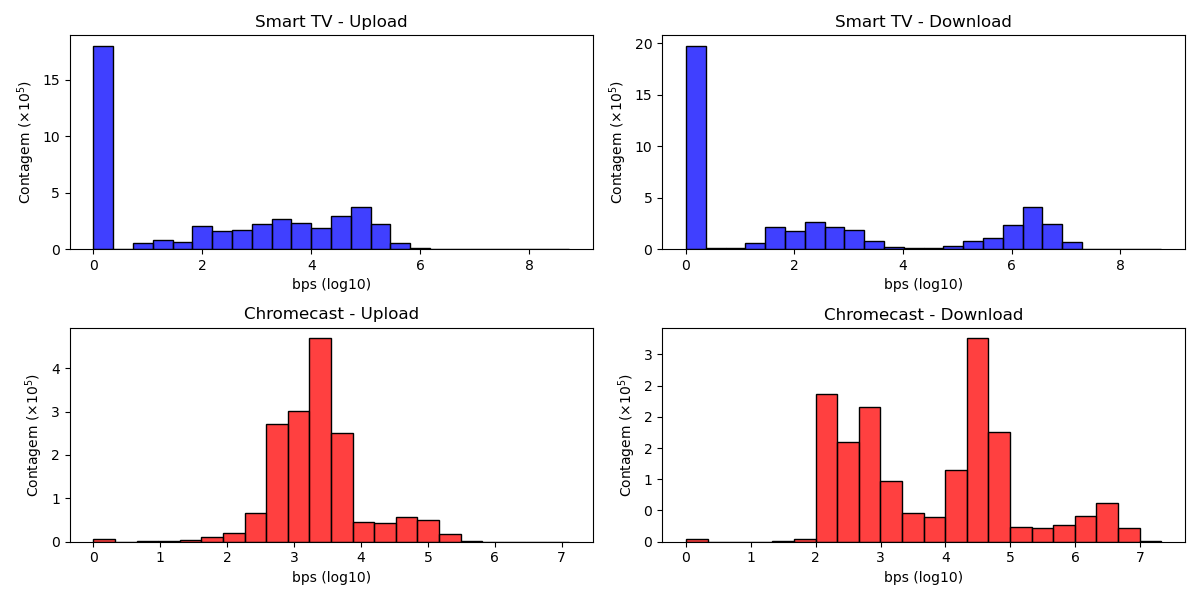
\includegraphics[width=0.8\textwidth]{../caracterizando os horários/histogramas.png}
    \caption{Histogramas das taxas de upload e download para os horários selecionados.}
    \label{fig:histogramas_horarios}
\end{figure}

\subsection{Passo 3: Estimativa de Parâmetros via MLE}

Os parâmetros das distribuições Gaussiana e Gamma foram estimados utilizando o método de Máxima Verossimilhança (\textit{Maximum Likelihood Estimation} - MLE) para os quatro conjuntos de dados. Esses valores foram aplicados na modelagem das distribuições, permitindo uma análise comparativa com os dados observados.

O MLE consiste em determinar os parâmetros que maximizam a função de verossimilhança, que mede a probabilidade dos dados observados para um conjunto de parâmetros. Para simplificar os cálculos, o logaritmo da verossimilhança (\textit{log-likelihood}) é utilizado. A derivada da \textit{log-likelihood} é igualada a zero para encontrar os estimadores de máxima verossimilhança dos parâmetros.

As funções de densidade de probabilidade para as distribuições Gaussiana e Gamma são definidas como:

\begin{itemize}
    \item \textbf{Gaussiana:}
    \begin{equation}
        f(x) = \frac{1}{\sigma \sqrt{2\pi}} e^{-\frac{(x - \mu)^2}{2\sigma^2}}
    \end{equation}
    onde \(\mu\) é a média e \(\sigma^2\) é a variância da distribuição.
    
    \item \textbf{Gamma:}
    \begin{equation}
        f(x) = \frac{\beta^\alpha x^{\alpha - 1} e^{-x/\beta}}{\Gamma(\alpha)}
    \end{equation}
    onde \(\alpha\) é o parâmetro de forma, \(\beta\) é o parâmetro de escala, e \(\Gamma(\alpha)\) é a função Gamma, definida como \(\int_0^\infty x^{\alpha - 1} e^{-x} dx\).
\end{itemize}

Para a distribuição Gaussiana, as estimativas dos parâmetros são obtidas de forma direta:

\begin{equation}
    \hat{\mu} = \frac{1}{n} \sum_{i=1}^{n} x_i, \quad \hat{\sigma}^2 = \frac{1}{n} \sum_{i=1}^{n} (x_i - \hat{\mu})^2
\end{equation}

No caso da distribuição Gamma, a estimação dos parâmetros \(\alpha\) (forma) e \(\beta\) (escala) pelo MLE não possui soluções analíticas simples e geralmente requer métodos numéricos iterativos. O parâmetro \(\alpha\) é frequentemente estimado utilizando o método de Newton-Raphson aplicado à função de log-verossimilhança, enquanto \(\beta\) pode ser estimado a partir de \(\alpha\) e da média amostral \(\bar{x}\) \cite{minka2002estimating}:

\begin{equation}
    \hat{\beta} = \frac{\bar{x}}{\hat{\alpha}}
\end{equation}

Para realizar essas estimativas, foi utilizado o método \texttt{gamma.fit} da biblioteca \texttt{scipy.stats} do Python. Este método aplica o MLE de forma eficiente, empregando algoritmos de otimização numérica para determinar os parâmetros que melhor se ajustam aos dados observados. Além dos parâmetros de forma (\(\alpha\)) e escala (\(\beta\)), o método também estima o parâmetro de localização (\(loc\)), que desloca a distribuição Gamma ao longo do eixo \(x\). Esse deslocamento é essencial quando os dados incluem valores iguais a zero (o que é o caso, como mostrado na Seção~\ref{sec:eda}), já que a função de densidade de probabilidade (PDF) da distribuição Gamma é indefinida para \(x = 0\) quando \(loc = 0\). Com \(loc > 0\), a PDF é modificada para começar em \(x = loc\), tornando possível ajustar a distribuição mesmo em presença de valores nulos ou muito baixos. A utilização desse parâmetro garante que a modelagem estatística permaneça válida e consistente com as características dos dados.


Os resultados das estimativas de parâmetros via MLE para as distribuições Gaussiana e Gamma são apresentados na Tabela~\ref{tab:resultados_mle}.

\begin{table}[H]
    \centering
    \caption{Resultados das estimativas de parâmetros via MLE}
    \label{tab:resultados_mle}
    \begin{tabular}{|c|c|c|c|c|c|}
        \hline
        \textbf{Dataset} & $\boldsymbol{\hat{\mu}}$ & $\boldsymbol{\hat{\sigma}^2}$ & $\boldsymbol{\hat{\alpha}}$ & $\boldsymbol{\hat{\beta}}$ & $\boldsymbol{\textit{loc}}$ \\ 
        \hline
        Dataset 1 (Smart TV - Upload) & 3.2243 & 3.1687 & 214.6171 & 0.1245 & -23.4982 \\ 
        \hline
        Dataset 2 (Smart TV - Download) & 3.4961 & 6.2013 & 883.8791 & 0.0838 & -70.5760 \\ 
        \hline
        Dataset 3 (Chromecast - Upload) & 3.6215 & 0.5957 & 3078.6394 & 0.0139 & -39.2307 \\ 
        \hline
        Dataset 4 (Chromecast - Download) & 4.1527 & 2.1594 & 27.1301 & 0.2832 & -3.5314 \\ 
        \hline
        \end{tabular}
    \end{table}

    Além disso, as \textit{log-likelihoods} e \textit{likelihoods} para as distribuições Gaussiana e Gamma são apresentadas na Tabela~\ref{tab:likelihoods}. As \textit{log-likelihoods} foram calculadas primeiro, para evitar erros de \textit{underflow} ao calcular as \textit{likelihoods}, substituindo a multiplicação de valores muito pequenos pela soma de seus logaritmos naturais.
    \begin{table}[H]
        \centering
        \caption{Likelihoods ($L$) e Log-likelihoods ($\log[L]$) para os Datasets}
        \label{tab:likelihoods}
        \begin{adjustbox}{center}
        \begin{tabular}{|c|c|c|c|c|}
        \hline
        \textbf{Dataset} & $\boldsymbol{\log[L]}$ \textbf{Gaussiana} & $\boldsymbol{L}$ \textbf{Gaussiana} & $\boldsymbol{\log[L]}$ \textbf{Gamma} & $\boldsymbol{L}$ \textbf{Gamma} \\ 
        \hline
        Dataset 1 (Smart TV - Upload) & -424282 & 0 & -427222 & 0 \\ 
        \hline
        Dataset 2 (Smart TV - Download) & -495658 & 0 & -495518 & 0 \\ 
        \hline
        Dataset 3 (Chromecast - Upload) & -89011 & 0 & -89015 & 0 \\ 
        \hline
        Dataset 4 (Chromecast - Download) & -129603 & 0 & -128993 & 0 \\ 
        \hline
        \end{tabular}
        \end{adjustbox}
    \end{table}

Os valores nulos das \textit{likelihoods} indicam que as distribuições propostas (Gaussiana e Gamma) não são adequadas para modelar os dados observados. Isso será visualizado melhor na próxima seção, onde os histogramas dos dados e as funções de densidade parametrizadas serão comparados.

\subsection{Passo 4: Gráficos de Densidade}

Gráficos contendo o histograma dos dados e as funções de densidade Gaussiana e Gamma, parametrizadas pelos valores obtidos no Passo 3, foram gerados utilizando o método \texttt{pdf} das classes \texttt{scipy.stats.norm} e \texttt{scipy.stats.gamma} do Python. Esses gráficos permitem uma comparação visual da aderência de cada distribuição aos dados reais e estão disponíveis na Figura~\ref{fig:histogramas_pdf}.

\begin{figure}[H]
    \centering
    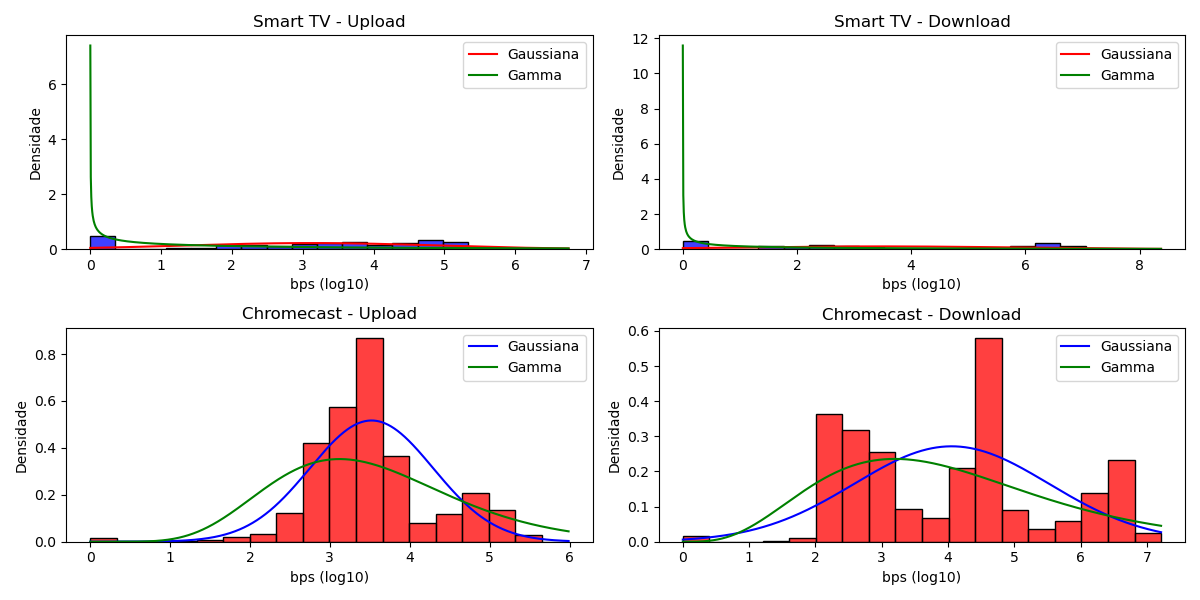
\includegraphics[width=0.8\textwidth]{../caracterizando os horários/histogramas_pdf.png}
    \caption{Histogramas dos dados e funções de densidade parametrizadas para as distribuições Gaussiana e Gamma.}
    \label{fig:histogramas_pdf}
\end{figure}

Observando a figura, é possível notar que nenhuma das distribuições propostas (Gaussiana e Gamma) se ajusta bem aos dados observados. Os histogramas sugerem que os dados não seguem uma distribuição normal e nem gamma, o que pode ser um dos motivos para a má aderência das distribuições propostas. A tabela de \textit{likelihoods} também indica que as distribuições propostas não são adequadas para modelar os dados, já que as \textit{log-likelihoods} são muito negativas, acarretando em \textit{likelihoods} nulas.

Uma sugestão seria utilizar uma mistura de distribuições para representar os dados, da seguinte forma:

\begin{itemize}
    \item \textbf{Dataset 1 (Smart TV - Upload):} Mistura de uma Gaussiana e uma Gamma.
    \item \textbf{Dataset 2 (Smart TV - Download):} Mistura de três Gaussianas.
    \item \textbf{Dataset 3 (Chromecast - Upload):} Mistura de duas Gaussianas.
    \item \textbf{Dataset 4 (Chromecast - Download):} Mistura de uma Gaussiana e duas Gammas.
\end{itemize}

Outra abordagem seria estimar a distribuição empírica dos dados, sem a necessidade de assumir uma distribuição paramétrica específica. Isso poderia ser feito utilizando métodos não paramétricos, como o estimador de densidade de Kernel (em inglês, \textit{Kernel Density Estimator} - KDE), que não requer a especificação de uma forma funcional para a distribuição dos dados. Utilizando o parametro KDE da biblioteca \texttt{seaborn} do Python, é possível estimar a distribuição empírica dos dados, como mostrado na Figura~\ref{fig:histogramas_pdf_kde}.

\begin{figure}[H]
    \centering
    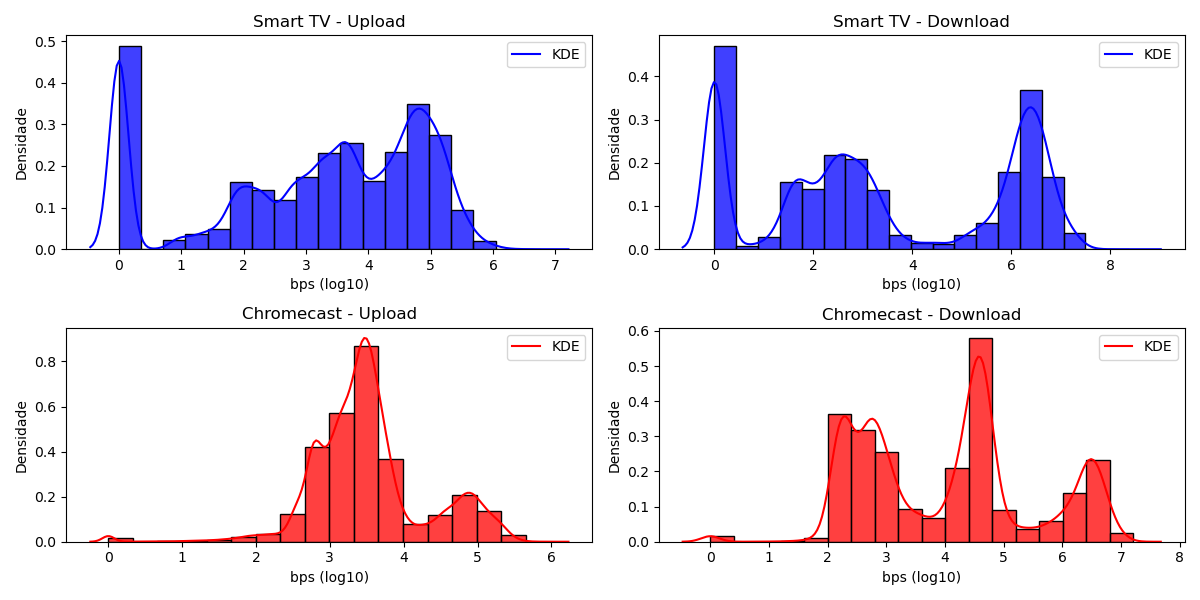
\includegraphics[width=0.8\textwidth]{../caracterizando os horários/histogramas_pdf_kde.png}
    \caption{Histogramas dos dados e estimativas de densidade empírica utilizando KDE.}
    \label{fig:histogramas_pdf_kde}
\end{figure}

\subsection{Passo 5: Probability Plots}

\textit{Probability Plots} foram criados para comparar os dados reais com as distribuições parametrizadas (Gaussiana e Gamma), utilizando o método \texttt{probplot} da biblioteca \texttt{scipy.stats} do Python.

No total, 8 gráficos foram gerados, permitindo avaliar a adequação das distribuições propostas aos dados. Essas gráficos podem ser observados nas Figuras~\ref{fig:probplot_gaussiana} e~\ref{fig:probplot_gamma}.

\begin{figure}[H]
    \centering
    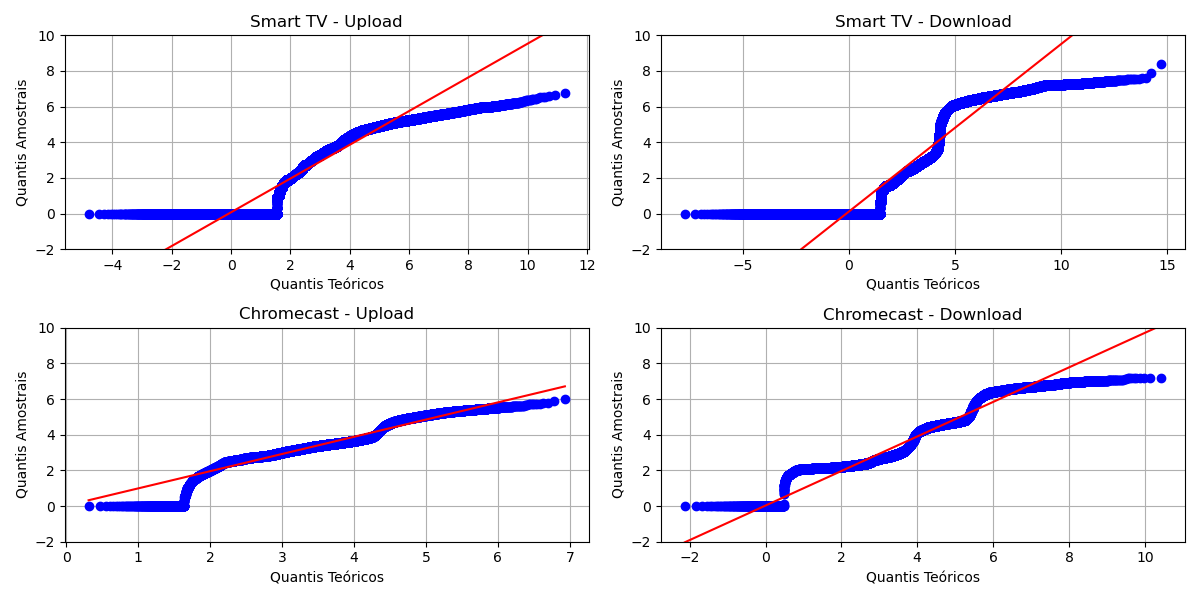
\includegraphics[width=0.8\textwidth]{../caracterizando os horários/probplot_gaussiana.png}
    \caption{Probability Plots para as distribuições Gaussiana.}
    \label{fig:probplot_gaussiana}
\end{figure}

\begin{figure}[H]
    \centering
    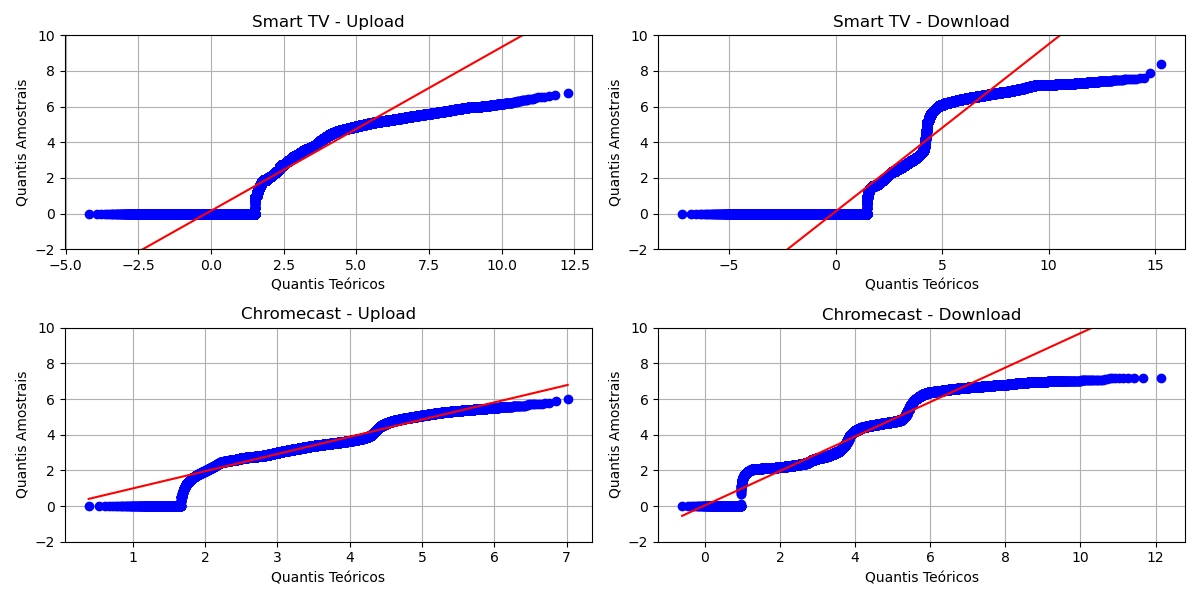
\includegraphics[width=0.8\textwidth]{../caracterizando os horários/probplot_gamma.png}
    \caption{Probability Plots para as distribuições Gamma.}
    \label{fig:probplot_gamma}
\end{figure}

A avaliação dos \textit{probability plots} revela que a distribuição Gaussiana apresenta um ajuste insatisfatório para todos os datasets analisados. Em todos os casos, observa-se que os pontos se distanciam consideravelmente da linha reta nas regiões extremas, com aproximação parcial na região central. No entanto, mesmo nessa aproximação, os pontos oscilam de forma significativa em torno da linha, indicando inconsistências no ajuste. A Gaussiana não consegue capturar a assimetria dos dados nem modelar adequadamente a alta concentração de valores baixos ou iguais a zero, como observado nas taxas de upload e download da Smart TV e do Chromecast.

A distribuição Gamma, apesar de ser mais flexível, também apresentou resultados insatisfatórios. Assim como a Gaussiana, os \textit{probability plots} mostram que a Gamma se distancia excessivamente da linha reta nos valores extremos e, embora se aproxime dela nos valores centrais, essa aproximação é marcada por oscilações significativas. Mesmo com o uso do parâmetro de deslocamento (\(loc\)) para lidar com os valores nulos, a distribuição Gamma não foi capaz de capturar a alta densidade de valores próximos de zero nem os padrões de dispersão observados. Dessa forma, ambas as distribuições falham em modelar adequadamente os dados analisados.
adequada que a Gaussiana para os dados analisados.


\subsection{Passo 6: QQ Plots}

\textit{QQ Plots} foram produzidos para comparar os datasets de upload e download entre os dispositivos (Smart TV e Chromecast). A interpolação linear foi utilizada para alinhar os quantis dos datasets de tamanhos diferentes. Esses gráficos permitem a análise das similaridades entre os padrões de tráfego dos dispositivos.

\subsection{Análise dos Resultados}

Com base nos resultados, as seguintes questões foram avaliadas:
\begin{enumerate}
    \item \textbf{Quais foram os horários escolhidos para cada dataset?}
    \item \textbf{O que foi observado a partir dos histogramas?}
    \item \textbf{Quais diferenças e/ou similaridades foram identificadas entre os datasets 1, 2, 3 e 4?}
    \item \textbf{É possível caracterizar os datasets por uma variável aleatória conhecida na literatura? Se não, por quê?}
    \item \textbf{O que foi observado a partir dos gráficos \textit{QQ Plot} e \textit{Probability Plot}?}
\end{enumerate}
% As conclusões são apresentadas em termos de suas implicações para o gerenciamento da rede e o entendimento dos padrões de tráfego para Smart TVs e Chromecasts.
